\documentclass[conference]{IEEEtran}
\IEEEoverridecommandlockouts
% The preceding line is only needed to identify funding in the first footnote. If that is unneeded, please comment it out.
\usepackage{cite}
\usepackage{amsmath,amssymb,amsfonts}
\usepackage{algorithmic}
\usepackage{graphicx}
\usepackage{textcomp}
\usepackage{xcolor}
\def\BibTeX{{\rm B\kern-.05em{\sc i\kern-.025em b}\kern-.08em
    T\kern-.1667em\lower.7ex\hbox{E}\kern-.125emX}}
\begin{document}

\title{Multipurpose Vertical Plotter Machine – MVPM\\
}

\author{\IEEEauthorblockN{ Sunilkumar Hattaraki}
    \IEEEauthorblockA{\textit{Department of Electronics and} \\
        \textit{Communication Engineering,}\\
        B.L.D.E.A’s V. P. Dr. P. G.  \\
        Halakatti College of Engineering \\
        and Technology, Vijayapur, India.\\
        Email:sunilmh039@gmail.com}

    % Second Author Name and Details

    \and
    \IEEEauthorblockN{Abhilsh Patil}
    \IEEEauthorblockA{\textit{Department of Electronics and} \\
        \textit{Communication Engineering}\\
        B.L.D.E.A’s V. P. Dr. P. G.  \\
        Halakatti College of Engineering \\
        and Technology, Vijayapur, India.\\
        E-mail:patilkumarabhi@gmail.com }

    % Third Author Name and Details

    \and
    \IEEEauthorblockN{Sujay Kulkarni}
    \IEEEauthorblockA{\textit{Department of Electronics and} \\
        \textit{Communication Engineering}\\
        B.L.D.E.A’s V. P. Dr. P. G.  \\
        Halakatti College of Engineering \\
        and Technology, Vijayapur, India.\\
        E-mail:sujayk928@gmail.com  }
}

\maketitle

\begin{abstract}
    The multipurpose vertical plotter machine is a
    device which functions as drawing or writing robot which
    designs images on wall, prints text on panel or board. It can
    be used for diverse applications like interior design, wall
    design, notice board writing and Advertisement design.
\end{abstract}

\vspace*{12pt}

\begin{IEEEkeywords}
    CNC Machine, Vertical plotting, 3 axis
    control, embedded system.
\end{IEEEkeywords}


\section{Introduction}
The present world is developing many technological
advancements in order to solve critical problems and issues in
an efficient way. It may be of reducing the resources use to
solve any kind of problem and making the process easier.
In context to this, we are creating a machine which helps to
solve complexities in different fields of plotting pictures, texts
and designs. Basically we are developing all in one vertical
plotter machine which can be used to plot on walls, boards and
panels in a flexible way.

\vspace*{12pt}

In order to establish this machine, we are using the Computer
numerical Control technology using which the several motors
are actuated to plot the design on the vertical panel. This CNC
technology helps in creating required designs on the software
and plotting that design on the XY plane with the help of
various motors.

\vspace{12pt}
Multipurpose vertical plotter machine works on the principle of
CNC (Computer Numerical Control) [2]. Multipurpose vertical
plotter machine basically works with two stepper motors and a
servo motor, the machine plots the design given to it from the
software on any vertical panel using Arduino which contains
ATMEGA328p microcontroller. The multipurpose vertical
plotter machine has control over all 3 axis [4], horizontal and
vertical control is done using stepper motors and servo motor is
used to control the z axis. Every axis motor is actuated by
arduino and a driver connected to it.

\vspace{12pt}

\vskip 55pt


A multipurpose vertical plotter machine eliminates many
disadvantages which are present in the conventional methods.
For designing any vertical panel like board or wall, the
conventional methods are highly depending on manual
procedure. The man made writing and designs probably have
less accuracy, poor quality and more error prone.

\vspace{12pt}

This machine is fully automatic and has computer based
designs so it comes with high precision, better quality and less
chance of error occurrence.

\vspace{12pt}

The plotters machines are predominantly horizontal plotters
which can only plot the design on horizontal axis, with the help
of plotter technology and adding verticality to its process fills
the requirement of automatic vertical plotting in an efficient
way.

\section{PROPOSED METHODOLOGY}
\vspace{12pt}
To establish this system we require different electronics
hardware and software elements

\vspace{12pt}

\subsection{Hardware:}
\begin{enumerate}
    \item Arduino UNO
    \item GRBL Shield
    \item Water Level Sensor
    \item Stepper Motors
    \item Servo Motor
    \item DC 12 volt 5A Rechargeable battery
\end{enumerate}
\subsection{Software:}
\begin{enumerate}
    \item Arduino IDE
    \item Universal G-code Sender
    \item Inkscape editor
\end{enumerate}


\clearpage


\subsection*{\textbf{A. Arduino UNO}}

\begin{figure}[h]
    \raggedright
    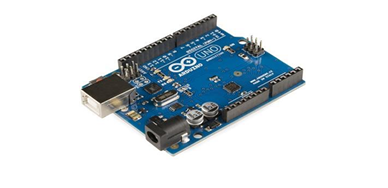
\includegraphics[width=0.4\textwidth]{arduino_uno_board.png}
    \caption{Arduino UNO board}
\end{figure}

One of the important device in our system is Arduino Uno. It is
a development board [5] which contains the ATmega328P
Microcontroller. It has 14 digital GPIO pins, 6 analogue IO
pins, a 16 MHz crystal oscillator, a USB port, a power jack, a
reset button and an ICSP header. The board has all the
supportive hardware for microcontroller; we just need to
connect it to a PC with a USB cable and supply the power.

Arduino is a core controller of this system, after creating the
design in G-code format, we upload that to Arduino board, we
connect GRBL shield to Arduino which acts as a driver to the
actuators, the G-code received by the Arduino is sent to GRBL
shield which eventually drives the stepper and servo motors.

\vspace{10pt}

\subsection*{\textbf{B. GRBL Shield}}


GRBL shield is used to make our system compatible with CNC
machine. It is an open source firmware which and mainly works
in the motion control for CNC machines. In simple words, the
GRBL software is uploaded to Arduino in order to control the
motors through Arduino. The above shown shield will be fit on
off arduino Uno which converts the G-code to motor motion.

\vspace{5pt}

\begin{figure}[h]
    \raggedright
    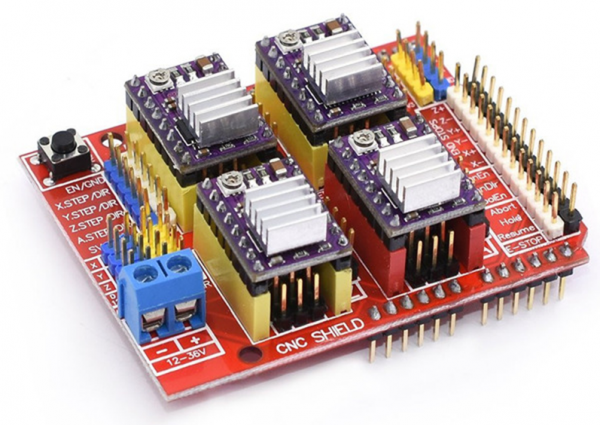
\includegraphics[width=0.35\textwidth]{grbl.png}
    \caption{GRBL Shield}
\end{figure}
The GRBL is very compatible to work with CNC machines
with low-cost small scale microcontrollers. It has its various
application with Arduino Uno, some of them are, laser
engraving/cutting machines, CNC milling machines, drawing
machines.


\subsection*{\textbf{C. Stepper Motors}}

\begin{figure}[h]
    \centering
    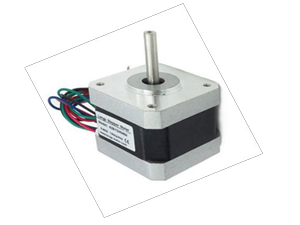
\includegraphics[width=0.3\textwidth]{motor.png}
    \caption{Stepper Motors}
\end{figure}

The stepper consist of rotor and coils, the rotor rotates when the
pulse input is given to the coils. The direction of the rotation
can be controlled by supplying the Pulse Width Modulated
signals which are controlled by the arduino board. Because of
its precise motion and high torque production in low power
supplies, it is very much suitable for our system. It has various
uses in low-cost and position control applications.

\vspace{5pt}
\subsection*{\textbf{D. Servo Motor}}

\begin{figure}[h]
    \centering
    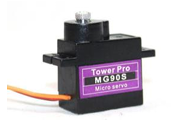
\includegraphics[width=0.3\textwidth]{servo.png}
    \caption{Servo Motor}
\end{figure}

The servo motor is DC motor uses very less power and
generates high precise degree rotations. When the electric
signal is provided to servo motor, it changes its mechanical
motion with accurate speed and direction control. In our system
we are using servo motor to control the z-axis. The end
effectors like pen or brush is connected to this motor, it holds
the pen up or down according to designing.

\subsection*{\textbf{E. Arduino IDE}}

\begin{figure}[h]
    \centering
    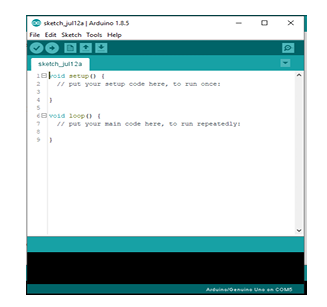
\includegraphics[width=0.20\textwidth]{arduino.png}
    \caption{Arduino IDE}
\end{figure}

The Arduino IDE (Integrated Development Environment)
is an environment used to write logic code according to our
system controlling requirements. It consists of an editor
window, text console and toolbar for different functions. The
environment is written in C and C++ functions. Initially we
write our code here, then connect the board to the computer and
upload all code to arduino board.

\subsection*{\textbf{F. Inkscape editor}}

\begin{figure}[h]
    \centering
    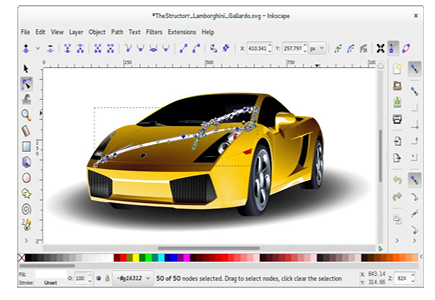
\includegraphics[width=0.40\textwidth]{ink.png}
    \caption{Inkscape editor}
\end{figure}

The CNC machine works on G-code input. Hence any kind of
design we want to draw need to be converted to G-code.
Inkscape software[7] provides the facility to construct the
design as per our requirement and convert it to G-code format.
In Inkscape we can create or edit graphics such as diagrams,
illustrations, line arts, charts, logos and complex paintings etc.

\subsection*{\textbf{G. Universal G-code Sender}}

\begin{figure}[h]
    \centering
    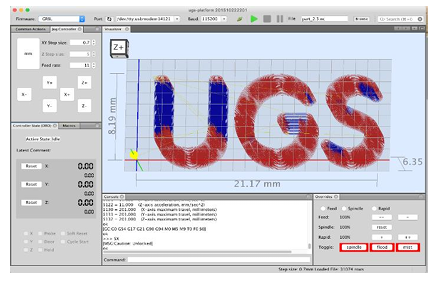
\includegraphics[width=0.40\textwidth]{universal.png}
    \caption{Universal G-code Sender}
\end{figure}

As name explains Universal G-code Sender is a platform used
to upload the G-code to the GRBL through arduino board. It is
a java application compatible with Windows, Mac OSX or
Linux.
\vspace{5pt}

The below block diagram and circuit diagram explains the
structure and working principle of the system.

\vspace{50pt}



\begin{figure}[t]
    \centering
    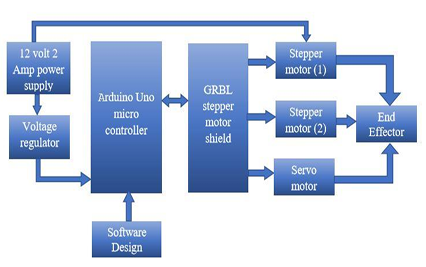
\includegraphics[width=0.60\textwidth]{block.png}
    \caption{Block diagram}
\end{figure}

The above figure shows the different blocks of the
multipurpose vertical plotter machine.

\vspace{5pt}
It has Arduino Uno as a core controller board which receives
the input commands from software and drives the motors. The
GRBL stepper motor shield will be connected on the top of the
Arduino board to which the stepper motor drivers are
connected.


\vspace{5pt}

It has two stepper motors and one servo motor. The stepper
motors are used to actuate the end effector in x and y axis and
servo motor to control in z- axis.

\vspace{5pt}


The 12 volt 2 amp supply is used to power up the stepper
motors. The voltage regulator provides constant 5V power
supply for Arduino Uno.

\vspace{5pt}

The following steps Explains the methodology and flow of
execution of the work.


\vspace{5pt}

1. Initially we create the required design on Inscape software
and generate the equivalent G-code of the design file. (.G
code).


\vspace{5pt}


2. Then we upload the working program to Arduino Uno
through Arduino IDE.


\vspace{5pt}


3. After generating the G-code in Incscape software we upload
this G-code to Arduino Uno using Universal G-code Sender
(UGC) software.


\vspace*{5pt}


4. When Arduino Uno receives the code commands, with the
help of GRBL shield, it actuates the stepper and Servo motors.


\vspace{5pt}


5: Because of movement of these motors, the end effector (e.g.:
marker, brush) writes the same design on any kind of vertical
panels like walls, boards etc.

\clearpage

\begin{figure}[h]
    \centering
    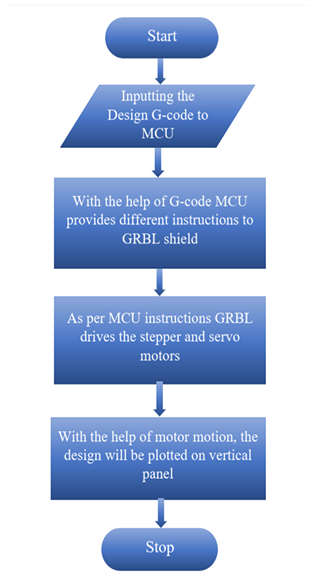
\includegraphics[width=0.35\textwidth]{work.png}
    \caption{Work flow}
\end{figure}
The virtual circuit connection is shown below:
\begin{figure}[h]
    \centering
    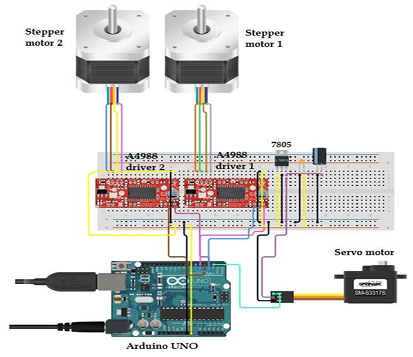
\includegraphics[width=0.40\textwidth]{circuit.png}
    \caption{circuit diagram}
\end{figure}

\vspace{90pt}

\section{RESULT AND DISCUSSION}

The main purpose of proposing this paper here is to bring up
the discussion that, using CNC technology, we can build a
machine which will be capable of designing anything on
vertical panel with slight modification in end effectors. We
have built the prototype of this machine which is shown below,
as a first stage we have designed it as a predominant writer as
we are connecting pen as end effector. But as we mentioned by
developing the design, we can use it for multi-purpose
applications like interior designing, designing of wall
advertisements etc.

\begin{figure}[h]
    \centering
    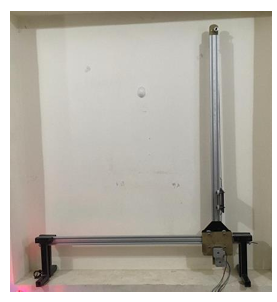
\includegraphics[width=0.35\textwidth]{prototype.png}
    \caption{Prototype of proposed machine}
\end{figure}

\vspace{5pt}
By studying the performance of the system, we can find
maximum advantages and few drawbacks.

\vspace{5pt}

\subsection*{\textbf{Advantages}}

\vspace*{5pt}
The CNC machine offers several advantages:

\begin{itemize}
    \item  The CNC machine works with high accuracy and acts as a robot, providing very high throughput.
    \item  Manual work is almost eliminated, reducing the chances of human error.
    \item  The machine has a high performance rate and requires less maintenance compared to manual processes.
    \item  Automatic handling of materials makes the manufacturing process more efficient and less labor-intensive.
    \item  The operation of the CNC machine is very reliable, ensuring consistent and precise results.
\end{itemize}
\vspace{15pt}
Initially to develop the machine it may require costly
components as application requirements and technically skilled
operators are required for handling of the machine. But these
can be considered as essential requirements rather than
drawbacks.


\clearpage

\section{CONCLUSION}

\vspace{5pt}
By observing the total system construction and working, we can
say the many problems regarding designs and writing can be
solved using this machine, as it is automatic, issues related to
human errors are eliminated, as it is a multipurpose device we
can include ma applications of designing. The conventional
plotter which plots only in horizontal axis is here used as
vertical plotter so as to fulfil our design requirements. Hence,
we can say that this multipurpose vertical plotter machine can
bring a change in vertical designing world



\vspace{5pt}

\section{References}
\vspace*{10pt}
\begin{enumerate}
    \item [1.] Al-Nahrain Journal for Engineering Sciences (NJES) Vol.21 No.3, 2018, pp. 350-355.
    \item [2.] Paulo A. Sherring da Rocha Jr., Rogério D. S. Souza and M. Emília de Lima Tostes, "Prototype CNC Machine Design," Journal of Energy and Power Engineering 6 (2012), 1884-1890, November 30, 2012.
    \item [3.] Kajal J. Madekar, Kranti R. Nanaware, Pooja R. Phadtare, Vikas S. Mane, "Automatic mini CNC machine for PCB drawing and drilling," International Research Journal of Engineering and Technology (IRJET), Volume: 03 Issue: 02, Feb 2016.
    \item [4.] Sundar Pandian, S. Raj Pandian, "A Low-Cost Build Your Own Three Axis CNC Mill Prototype," International Journal on Mechanical Engineering and Robotics (IJMER), Volume-2, Issue-1, 2014.
    \item [5.] W. Durfee, "Arduino Microcontroller Guide," University of Minnesota, ver. Oct-2011.
    \item [6.] https://www.arduino.cc/en/guide/Environment
    \item [7.] https://www.inkscape.org
    \item [8.] https://github.com/martymcguire/inkscape-unicorn
    \item [9.] https://processing.org/download
\end{enumerate}








\end{document}